\section{Register Allocation}

The annotated CFG and the associated interference graph are shown below. 

We first identify the live ranges of all the variables. We split
pseudo-registers into live ranges to create an interference graph that
is easier to color.

We observe that the graph has a 5-clique comprising of $\{y, x_2, s_1, t, u \}$.
Hence, there is no possible 4-coloring for the graph.

We then compute the spilling cost for all the variables involved in the clique.
We note that either $x_2$ or $u$ can be spilled with minimal cost.
After spilling, say $u$, we provide a 4-coloring of the graph in the figure.
Thus, it is possible to allocate the variables in this case to 4 physical
registers after spilling $u$.

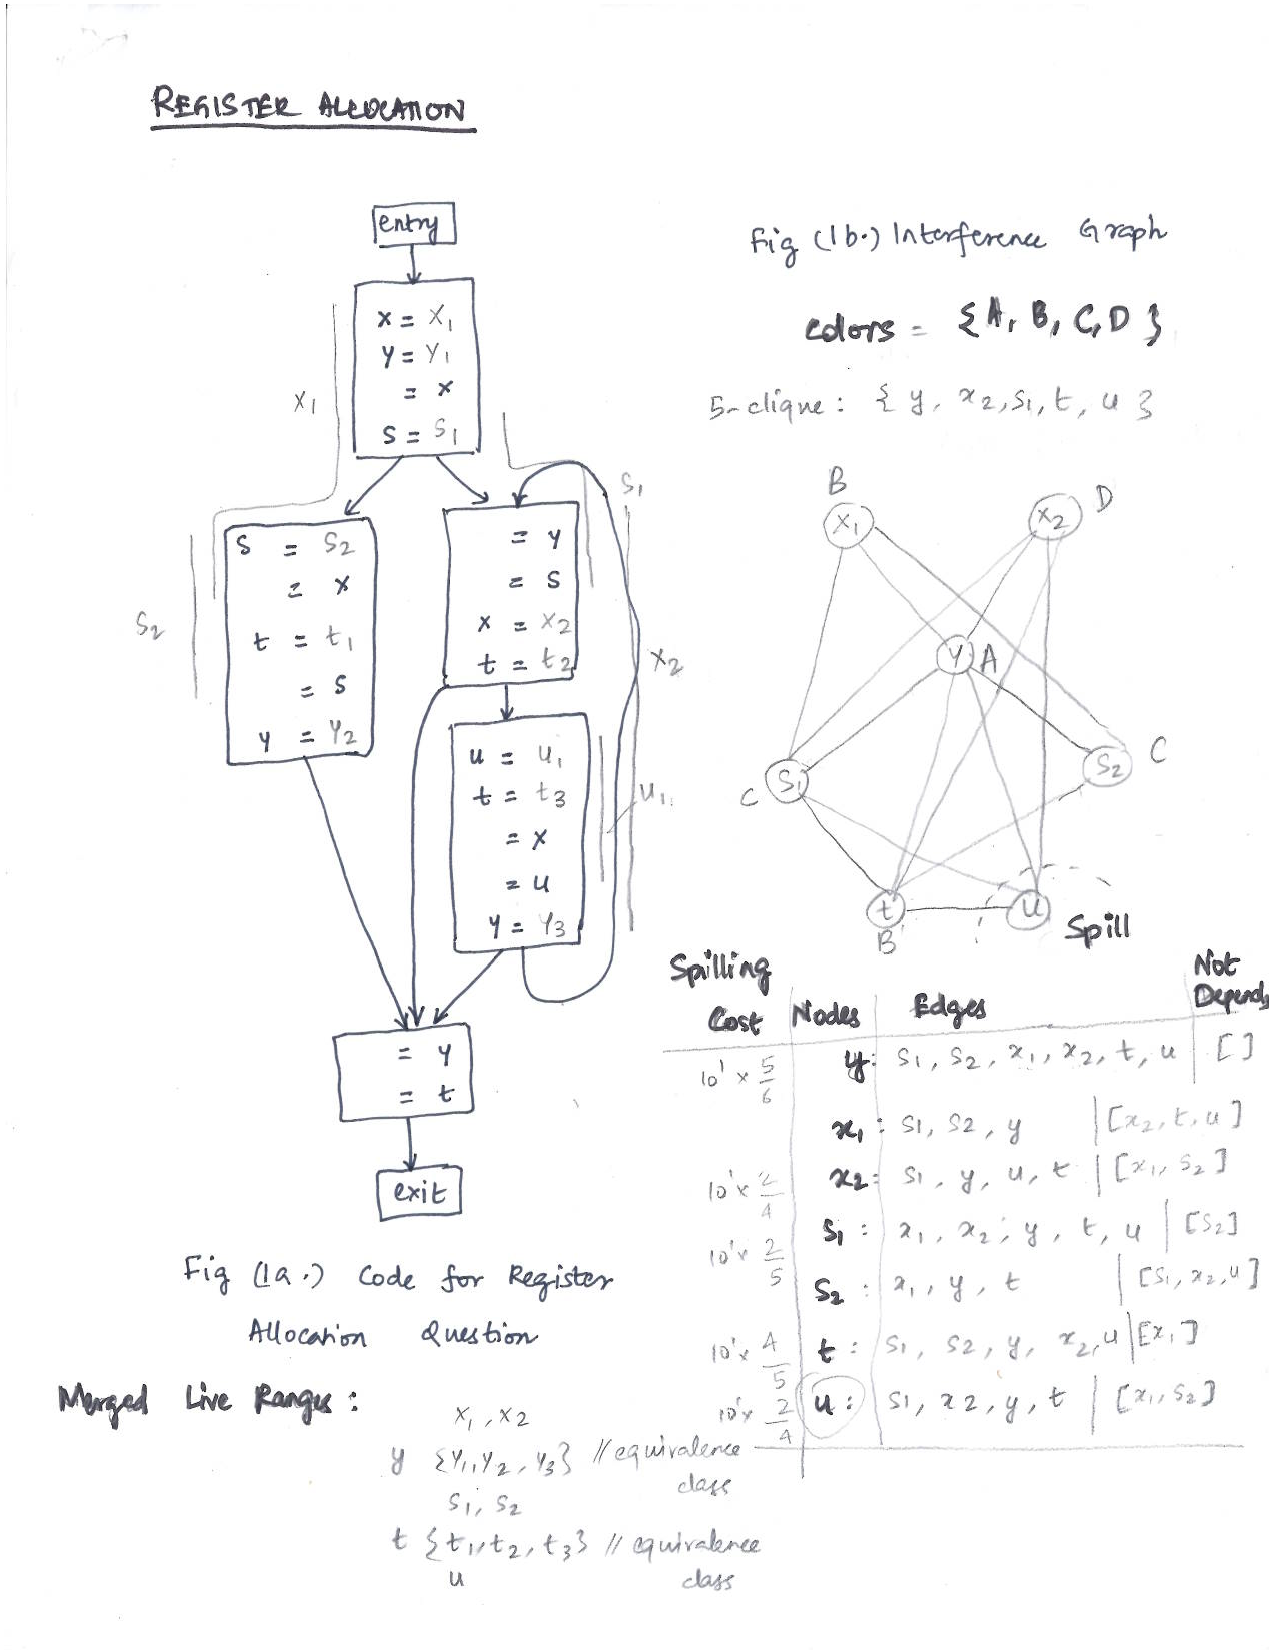
\includepdf[scale=0.7, pages={-}]{images/Q2.pdf}
